\section{Kablolu drone platformlarıyla seçmeli elma hasadı}\label{sec:harvest}

Kıyaslamada tamamlanma süresi sabit bir bütçede ölçülmüştür. Bir hasat operasyonunda ise plan,
bir platform kasa değişimi için her döndüğünde yeniden hesaplanır, ağaç başına meyve
sayıları ağaçlar gözlemlenene kadar belirsiz kalır ve hareket sıra aralarıyla
sınırlıdır. Bu bölümde planlayıcılar, böyle bir operasyonun ayrık olaylı benzetiminde
değerlendirilmiştir; benzetim parametreleri, değer bulunabilen her durumda
tarım literatüründen alınmıştır.

\subsection{Senaryo}

\begin{figure}[t]
\centering
\begin{minipage}{0.485\textwidth}\centering
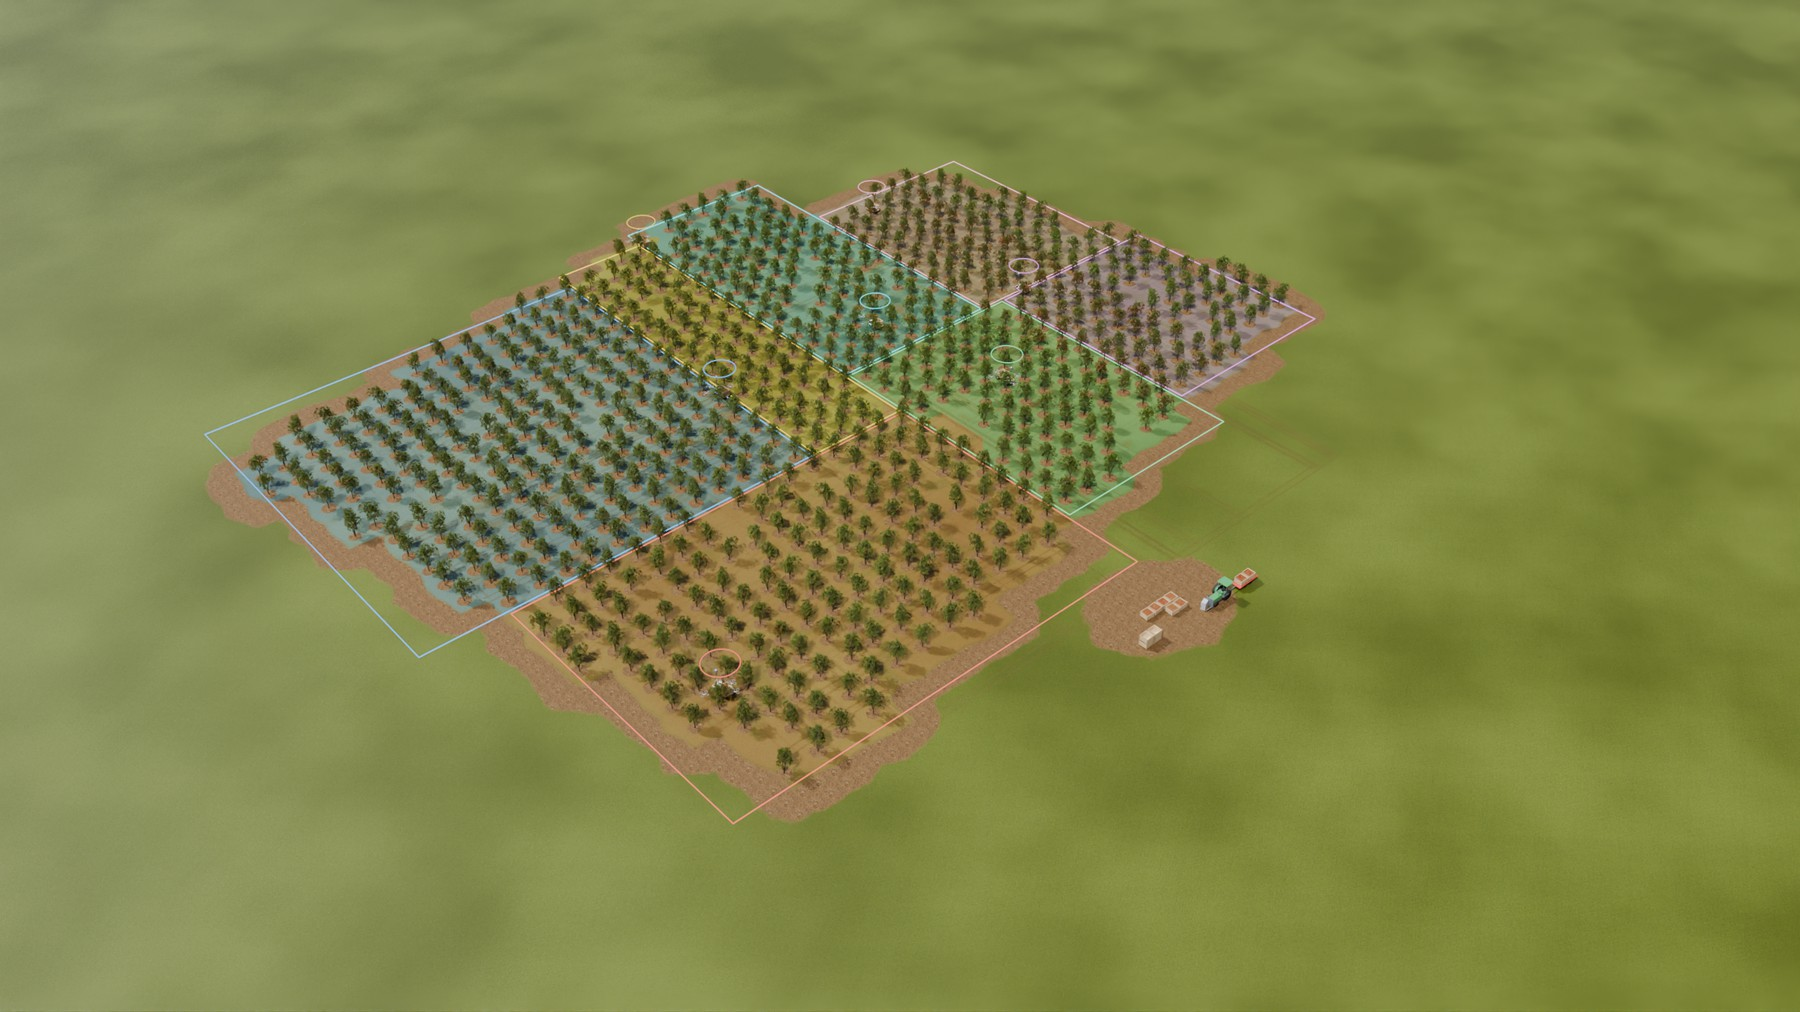
\includegraphics[width=\linewidth]{figs/fig_v4_overview.jpg}\\(a)
\end{minipage}\hfill
\begin{minipage}{0.485\textwidth}\centering
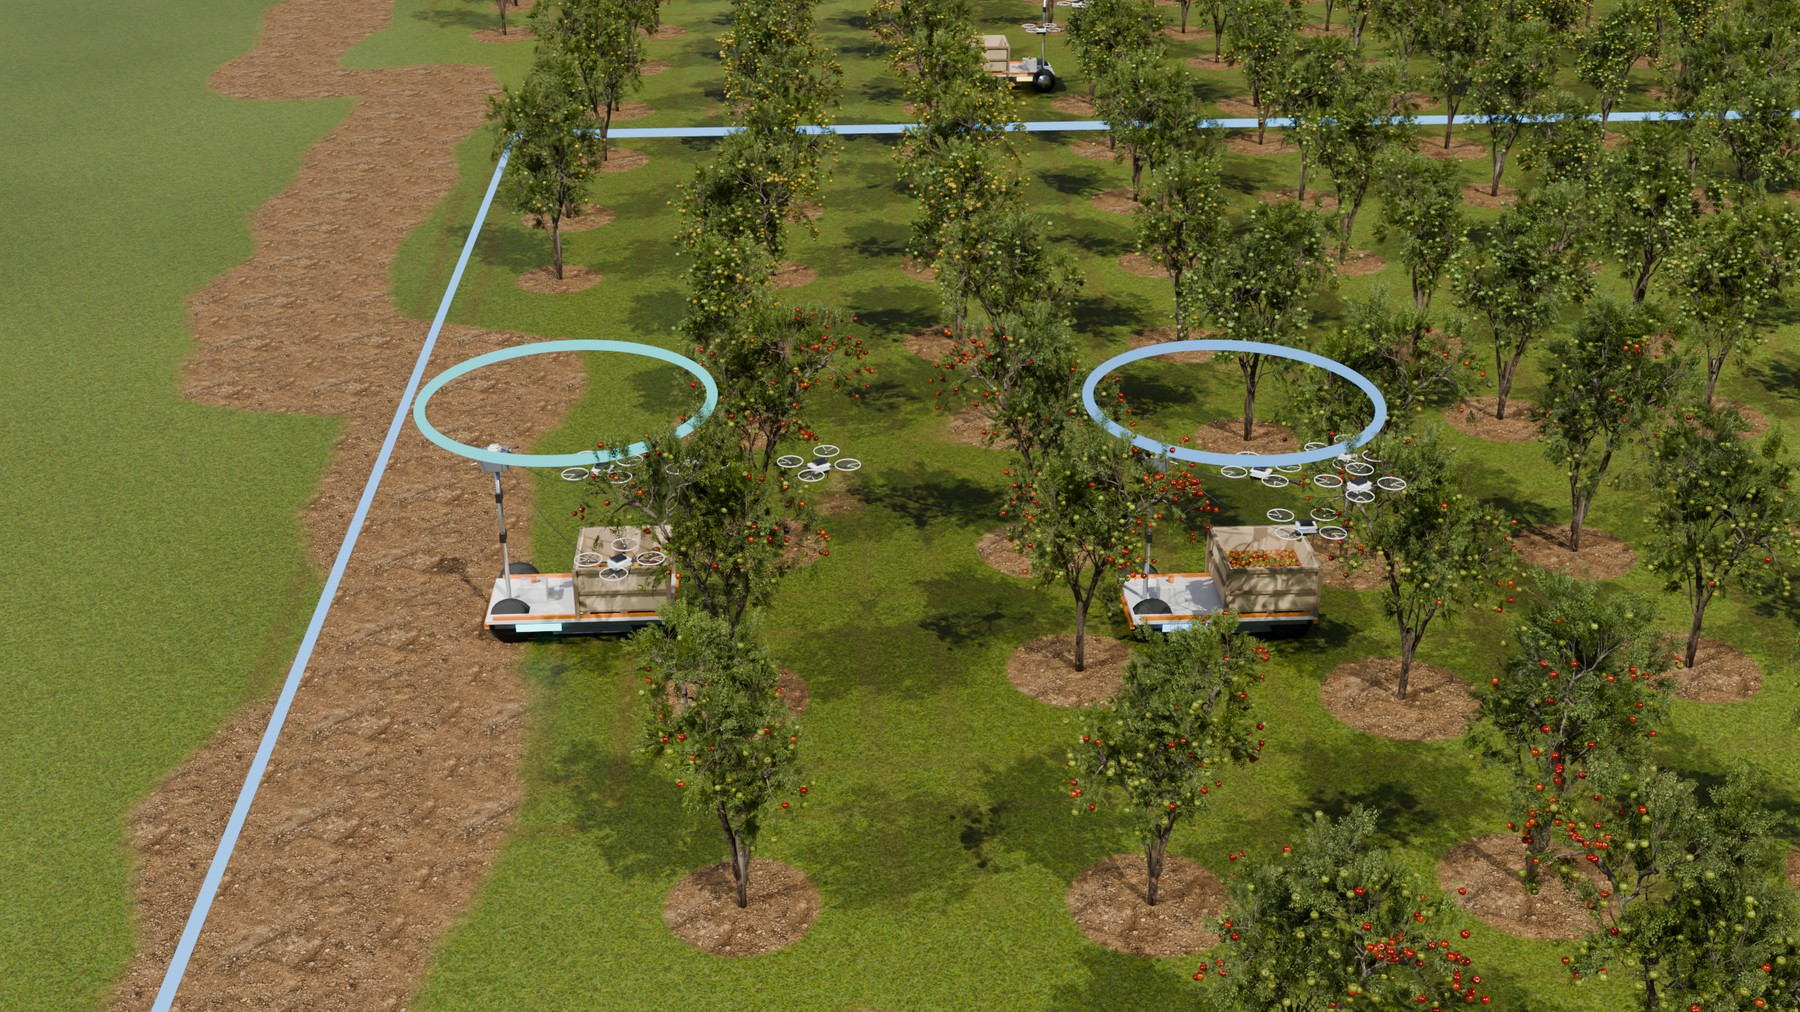
\includegraphics[width=\linewidth]{figs/fig_v4_takeover.jpg}\\(b)
\end{minipage}\\[4pt]
\begin{minipage}{0.485\textwidth}\centering
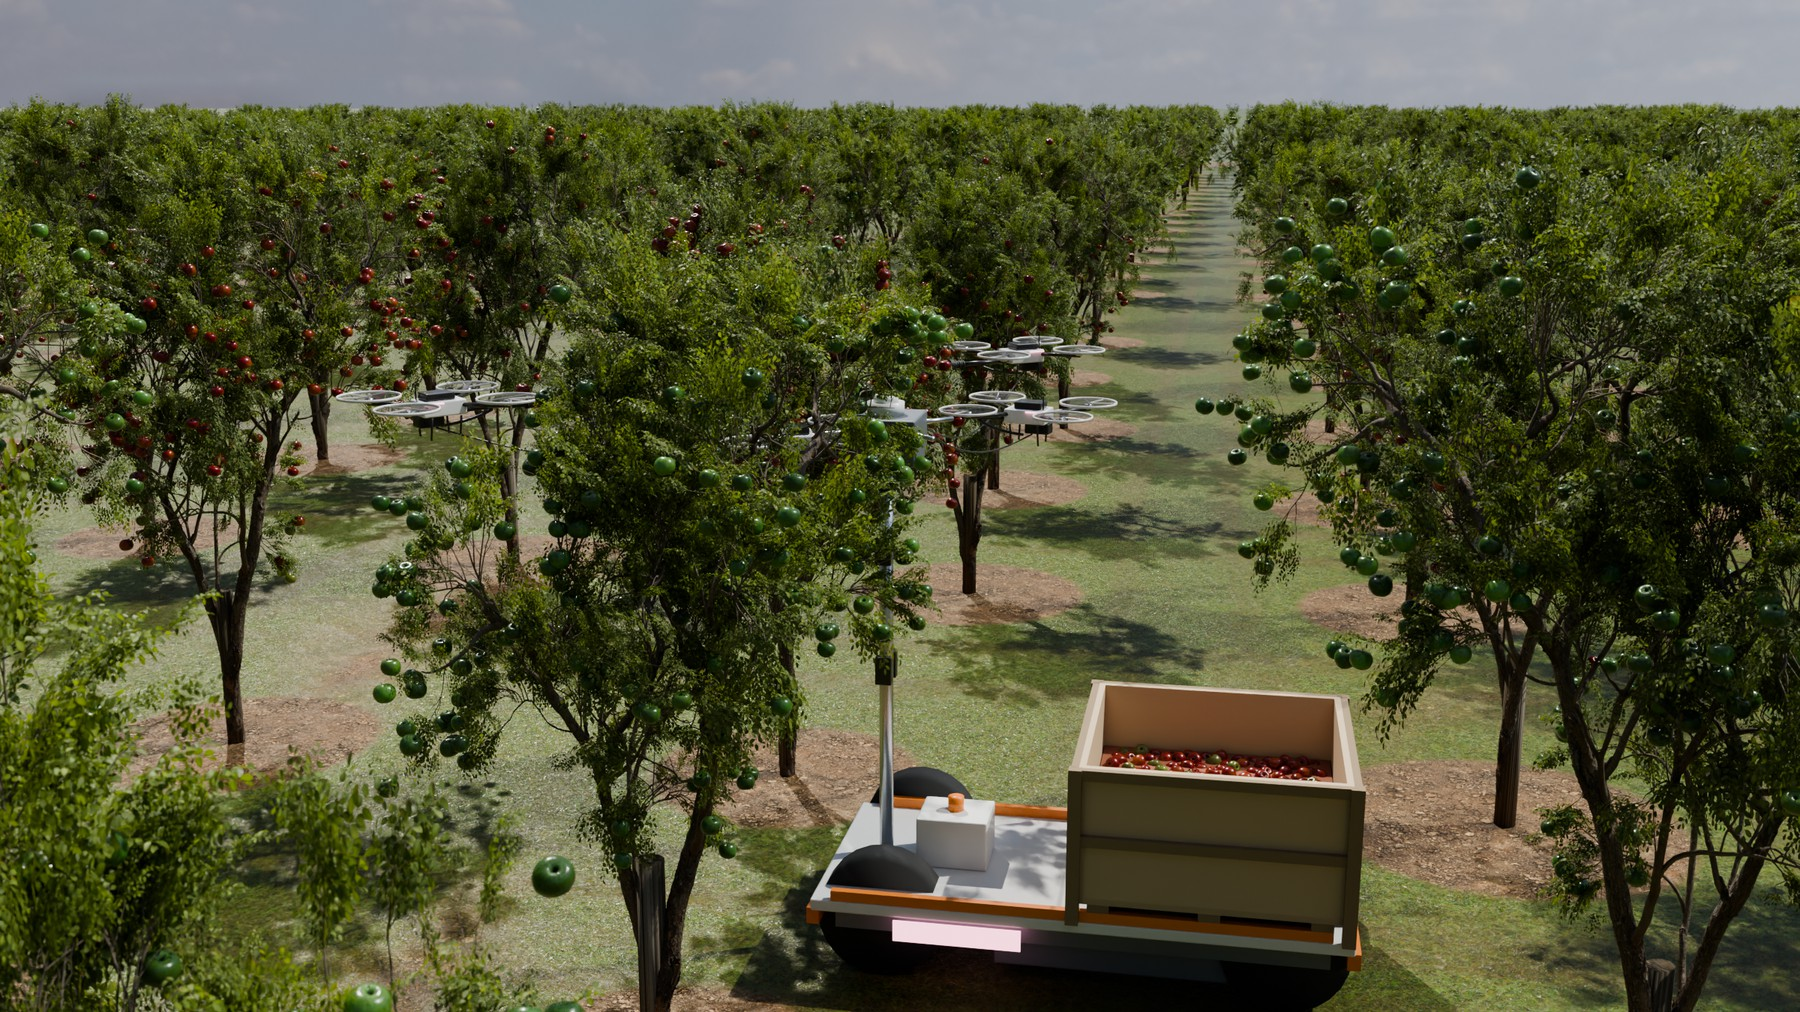
\includegraphics[width=\linewidth]{figs/fig_v4_platform.jpg}\\(c)
\end{minipage}\hfill
\begin{minipage}{0.485\textwidth}\centering
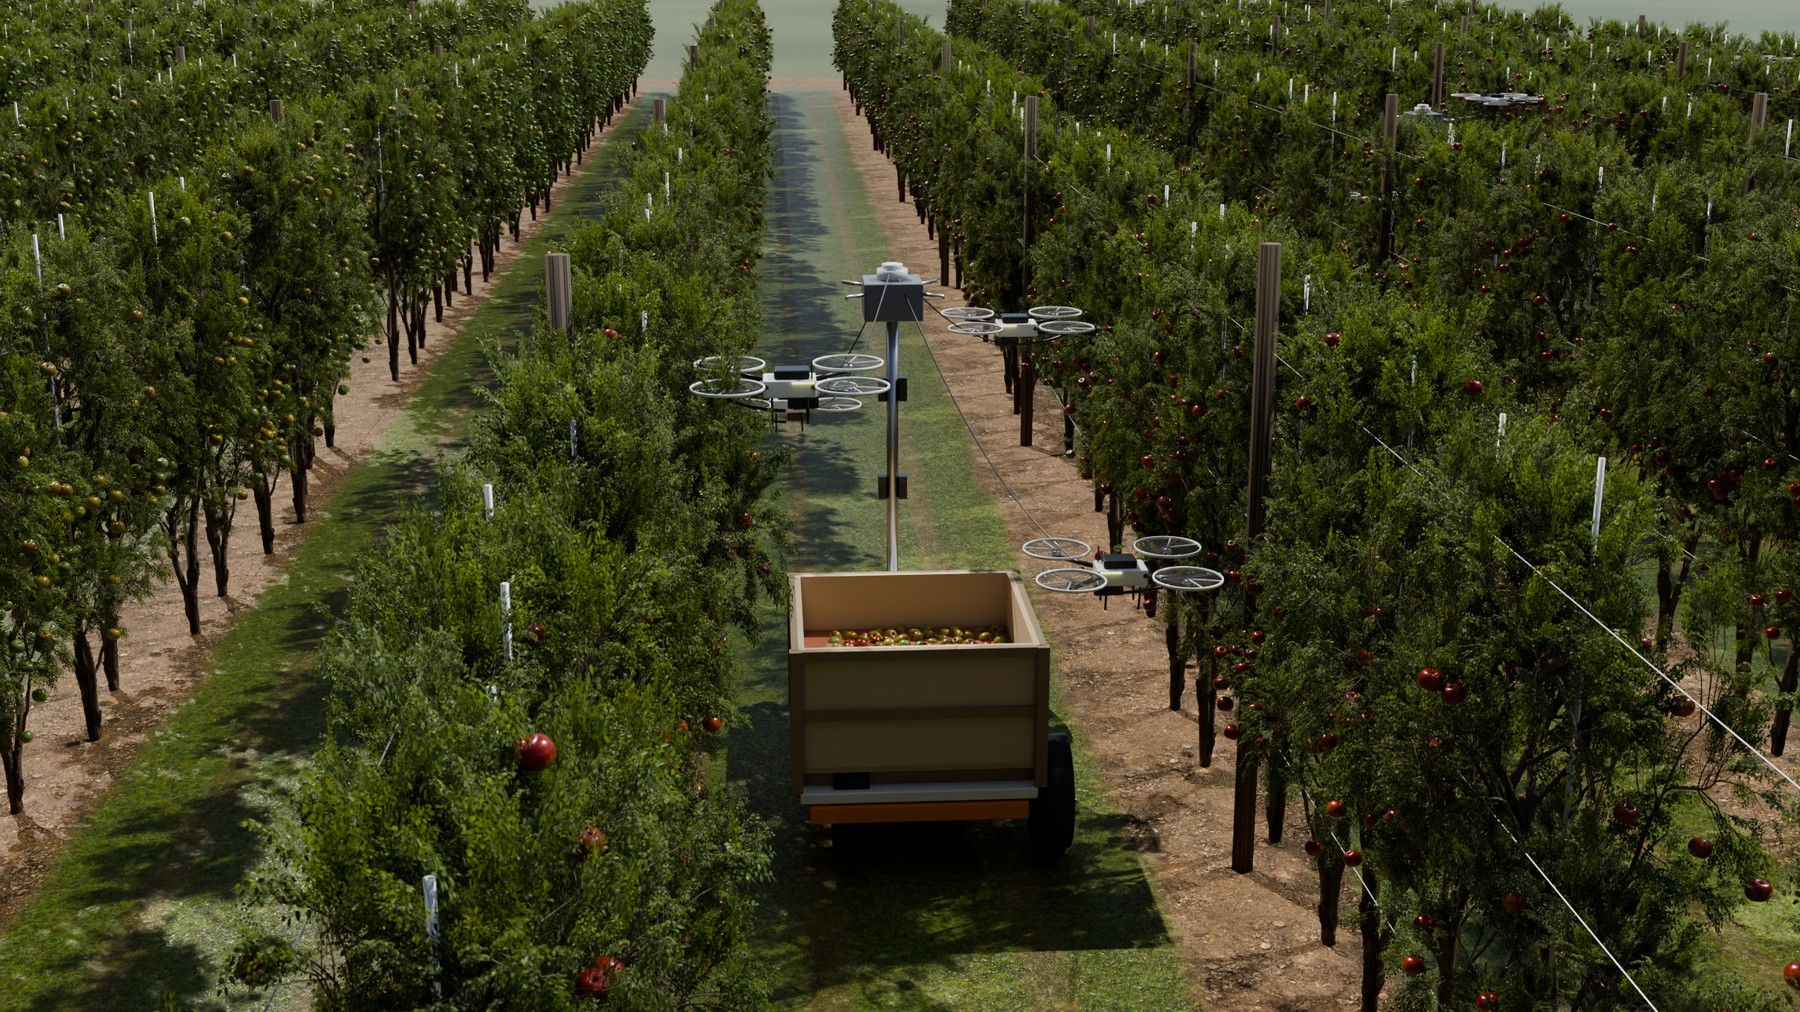
\includegraphics[width=\linewidth]{figs/fig_v3_platform.jpg}\\(d)
\end{minipage}
\caption{Benzetimi yapılan görevlerin yeniden oynatımı: (a) $k$-d bölgeleriyle kare dikimli
bahçe; (b) uç devralma; (c) bir sıra arası kesişiminde dört kablolu drone taşıyan
platform; (d) Tall Spindle bahçesi}\label{fig:blender}
\end{figure}

Benzetimde, her biri bir kasa ile dört drone'un kabloyla bağlandığı bir merkez birimi taşıyan
yer platformlarından oluşan bir filo modellenmiştir (Şekil~\ref{fig:blender}); bu kurgu, sektör
basınında tanıtılan kablolu meyve toplama robotlarından esinlenmiştir \citep{oitzman_2021_tevel,coxworth_2022_fruitpicking}.
Bu tür sistemlere ilişkin hakemli performans verisi bulunmadığından, sistem parametreleri
duyarlılık analizinde değiştirilmiştir. Senaryo, taze tüketim pazarına yönelik seçmeli
bir toplamadır: yalnızca olgun meyveler toplanır ve kasaya yerleştirilir. Taze tüketime
yönelik elmalar küçük düşme yüksekliklerinde bile ezildiğinden \citep{schulte_1992_apple}
ve yere temas ettikten sonra taze tüketim için satılamadığından \citep{ewing_2018_food},
meyvenin düşürülmesi bu elmalar için bir seçenek değildir; sanayilik elmalar ise sıra
üstü sarsıcılarla çok daha hızlı hasat edilmektedir \citep{brawner_2025_overtherow}; bu nedenle
seçmeli drone hasadı yalnızca taze tüketim pazarı için anlamlıdır.

\subsection{Model}

\begin{table}[t]
\centering
\caption{Benzetim parametreleri. ``Varsayım'' ifadesi, ölçülmüş karşılığı bulunamayan
değerleri belirtir; duyarlılık analizi, aralık sütununda değer verilen parametrelerle
ve her seferinde tek parametre değiştirilerek sınırlandırılmıştır}\label{tab:params}
\scriptsize
\begin{tabular}{p{3.3cm}p{2.4cm}p{1.8cm}p{3.4cm}}
\toprule
parametre & değer & duyarlılık aralığı & kaynak \\
\midrule
\multicolumn{4}{l}{\emph{Bahçe}} \\
kare dikim aralığı & 4.0\,m $\times$ 4.0\,m ($\pm$5--10\%) & 3.5--5.0\,m & düşük yoğunluklu serbest duran sistemler \citealp{brawner_2026_wsu,robinson_2008_evolution} \\
Tall Spindle (sıralı bahçe durumu) & 0.9\,m $\times$ 3.3\,m & -- & \citealp{robinson_2011_tallspindle,hoying_nd_tallspindle,reig_2020_longterm} \\
konum gürültüsü, bükülmüş sıralar, boşluklar & 0.25\,m; 0.2--0.6\,m; 6\% + öbekler & 0.1--0.6\,m & varsayım \\
ağaç başına meyve (kare dikim; sıralı) & NB ortalaması 300; 130 & 150--450 & \citealp{francescatto_2020_precision} \\
meyve sayısı saçılımı / hedef eşiği & NB $r=5$ / 5 olgun meyve & -- & varsayım \\
çeşit, uzamsal alan ve meyve gürültüsü & üç kayma; 0.35; 0.35 & -- & varsayım \\
bir toplama geçişinde olgun meyve payı & 40\% (ilk), 15\% (seyrek) & -- & \citealp{simnitt_2023_advancements,hall_2001_effect}; varsayım \\
dış/üst meyvelerin daha erken olgunlaşması & evet & -- & \citealp{roper_2001_when,moran_2022_honeycrisp}; aksi yönde \citealp{kviklys_2022_apple} \\
\midrule
\multicolumn{4}{l}{\emph{Algılama ve toplama}} \\
ön kestirim hatası & log-normal, $\sigma=0.6$ & 0.3--0.9 & varsayım \\
geçiş sırasında görünür meyve payı & 0.60 & -- & \citealp{gongal_2016_apple} (vekil ölçüt) \\
tespit yakalama oranı / kesinlik & 0.85 / 0.88 & yakalama oranı 0.82--0.97 & \citealp{kang_2020_fast,sapkota_2024_comparing,genemola_2020_fruit} \\
girişim başına koparma başarısı & 0.80 & -- & \citealp{silwal_2017_design,zhang_2024_automated,zhu_2025_advancement} \\
toplama girişimi başına süre & 6.0\,s & 3.6--7.3\,s & \citealp{silwal_2017_design,zhang_2024_automated,hohimer_2019_design} \\
platform başına drone sayısı & 4 & 2--6 & \citealp{oitzman_2021_tevel,coxworth_2022_fruitpicking} (sektör basını) \\
\midrule
\multicolumn{4}{l}{\emph{Platform ve lojistik}} \\
sıra aralarında platform hızı & 1.0\,m/s & 0.5--2.0\,m/s & varsayım \\
durma / dönüş süresi & 20\,s / 20\,s & -- & varsayım \\
kasa kapasitesi & 2300 meyve ($\approx$380\,kg) & 1500--3000 & varsayım \\
istasyonda kasa değişim süresi & 120\,s & 60--300\,s & varsayım \\
\bottomrule
\end{tabular}

\end{table}

\paragraph{Bahçeler} Ana durum, platformların sıra aralarında her iki yönde de
ilerleyebildiği, serbest duran ağaçlardan oluşan kare dikimli bir bahçedir (yaklaşık
4\,m'ye 4\,m). Geometri bilinçli olarak kusurlu tutulmuş ve her tohumla değiştirilmiştir:
iki yöndeki aralıklar birbirinden 5--10\% farklıdır, sıralar 0.2--0.6\,m'lik düşük
frekanslı bir yer değiştirmeyle bükülmüş, her ağaç $\sigma=0.25$\,m standart sapmayla kaydırılmış,
ağaçların 6\%'sı rastgele çıkarılmış ve en fazla üç ölü ağaç öbeğiyle ek ağaçlar
kaldırılmıştır; sınır olarak ya çentikli 1.3\,ha'lık bir blok ya da Şekil~\ref{fig:osm}'deki
dört gerçek bahçe sınırından biri (1.0 ile 5.4\,ha arası) kullanılmış, bahçenin yönelimi ise planlayıcılara
bildirilmemiştir. Bahçelerde \HgTreesMin{} ile \HgTreesMax{} arasında ağaç
bulunmaktadır. Bu geometri, Isparta'nın en çok elma üreten ilçesi olan Gelendost'taki
\citep{sargin_2014_isparta} bahçelerin herkese açık uydu görüntüleriyle karşılaştırılmıştır
(ör. 38.125\,K, 31.025\,D). İncelediğimiz parsellerde hem kare dikimli (ağaç aralığı yaklaşık 5\,m)
hem de sıralı bahçeler yer almakta ve parsellerin çoğu 1\,ha'dan küçüktür. Benzetimdeki bahçeler
ise daha sık dikimli (4\,m) ve daha büyüktür; bükülmüş sıralar, eksik ağaçlar ve çentikli sınırlar
da bilinçli olarak belirgin tutulmuştur. Dolayısıyla benzetim, ağaç sayısı ve geometrik düzensizlik
bakımından bu bahçelerden daha zorlayıcıdır. İkinci durumda, dört sınır üzerinde yüksek yoğunluklu bir Tall Spindle
dikimi (0.9\,m'ye 3.3\,m) kullanılmıştır; bu durumda platformlar sıra aralarında kalmak zorundadır
ve bir sıra arasından diğerine baş tarla üzerinden geçer.

\paragraph{Meyve ve algılama} Kare dikimli ve sıralı bahçelerde ağaç başına
meyve sayısı sırasıyla $\mu=300$ ve $130$ olmak üzere
$N_i\sim\mathrm{NB}(5,5/(5+\mu))$ dağılımından üretilmiştir. Meyve $\ell$'nin
olgunluk puanı
$m_{i\ell}=b_{c(i)}+0.35z_i+0.45(U_{i\ell}-0.5)+\varepsilon_{i\ell}$,
$\varepsilon_{i\ell}\sim N(0,0.35^2)$ biçimindedir; $b_{c(i)}$ beş sıralık
bloklara atanan üç çeşidin kayması, $z_i$ on iki rastgele Gauss tepesinden oluşan,
standartlaştırılmış uzamsal alan ve $U_{i\ell}\sim U(0,1)$ dış/üst konum
avantajıdır. $m\ge0$ olan meyve olgun sayılmıştır. İlk geçişte çeşit kaymaları
$(0.148,-0.202,-0.602)$, seyrek geçişte $(-0.291,-0.641,-1.041)$ alınarak
hedef olgun payları yaklaşık \%40 ve \%15 olarak kalibre edilmiştir.

$R_i>0$ için ilk kestirim $R_i\exp(N(0,0.6^2))$, $R_i=0$ için Poisson(2)
değeridir. Kameralar 10\,m içindeki ağaçları gözler; gözlenen ağacın kestirimi,
$X_i\sim\mathrm{Binomial}(R_i,0.60)$ olmak üzere $X_i/0.60$ ile güncellenir.
Bu büyüklük doğrudan görünür meyve sayısı değil, görünürlük düzeltilmiş toplam
olgun meyve kestirimidir. Ziyaret edilen ağaçta tespit sayısı
$D_i\sim\mathrm{Binomial}(R_i,0.85)$ olup ham meyve girişimleri, gerçekleşen
$D_i$ ve tespit kesinliği 0.88'e göre üretilir; her girişim bağımsız olarak 0.80
olasılıkla başarılıdır. Durak süresi, 20\,s durma süresi ile girişim sayısının
6\,s/drone sayısıyla çarpımının toplamıdır. Kasa dolarsa durak bölünür ve ağaç
daha sonra yeniden ziyaret edilir; aksi hâlde ağaç işlenmiş sayılır. Kestirimi en
az beş olgun meyve olan ve henüz işlenmemiş veya başka bir seferde ayrılmamış
ağaçlar hedef havuzunu oluşturur; görev bu havuz boşaldığında ve süren seferler
tamamlandığında sona erer.

\paragraph{Planlayıcılar} Tüm planlayıcılarda aynı kestirimler ve aynı kasa kuralı kullanılmıştır.
\emph{PSB-MT/R}, her kasa değişiminde tüm filonun kalan işini, \nameref{sec:ext} bölümünde açıklanan
bahçe eksenine duyarlı dev tur, kapasiteli bölme ve atama adımlarıyla yeniden planlar.
\emph{k-d+TO} uç devralmalı $k$-d bölgelerini, \emph{k-d} ise aynı bölgeleri devralma
olmaksızın kullanır. \emph{OR-Tools}, aynı $L_1$ yol süreleri ve hizmet süreleriyle tanımlanan
kapasiteli bir rotalama problemini yönlendirmeli yerel arama (guided local search) ile
çözer (yeniden planlama başına 1\,s) ve seferleri PSB-MT/R'deki gibi atar.
\emph{Açgözlü dağıtım}, dönen bir platformu kasasının dolduğu kestirilene kadar en yakın
ağaçlara gönderir. Basit bir statik alan bölümleme referansı olan \emph{sıra bantları}
yöntemi, tüm ağaç dizilerinin yılan biçimli sıralamasını kestirilen işi eşit olan
$k$ bitişik parçaya böler ve yeniden planlama yapmaz. Bahçe ekseninin rolünü
yalıtmak amacıyla PSB-MT/R harita eksenleriyle, k-d+TO ise ayrıca gerçek eksenlerle
(\emph{kâhin}) ve harita eksenleriyle çalıştırılmıştır.
Filo büyüklüğü, ilk toplama geçişinin kestirilen işi yaklaşık altı saat sürecek şekilde
seçilmiştir (\HgKMin{} ile \HgKMax{} arası platform); beş bahçe ve iki geçişin her
birinde beş ortak tohum kullanılarak planlayıcı başına 50 eşleştirilmiş koşu elde
edilmiştir. Parametreler Tablo~\ref{tab:params}'de listelenmiştir.

\subsection{Bulgular: kare dikimli bahçeler}

\begin{table}[t]
\centering
\caption{Kare dikimli bahçeler: beş tohum üzerinden ortalama görev süresi [h]; kalın: her
satırdaki en iyi değer. k-d+TO: uç devralmalı $k$-d bölgeleri}\label{tab:hgrid}
\footnotesize
\setlength{\tabcolsep}{4pt}
\begin{tabular}{lrrrrrr}
\toprule
orchard & k-d+TO & k-d & PSB & OR-Tools & greedy & row bands \\
\midrule
\multicolumn{7}{l}{\emph{first pick (40\,\% ripe): mission time [h], mean of 5 seeds}} \\
notched 1.3 ha block ($k=7$) & 5.49 & 5.82 & \textbf{5.34} & 5.37 & 5.56 & 5.66 \\
real 1.0 ha ($k=6$) & 5.51 & 5.88 & \textbf{5.32} & 5.33 & 5.49 & 5.47 \\
real 2.0 ha ($k=11$) & 6.44 & 6.76 & \textbf{6.05} & 6.20 & 6.45 & 6.40 \\
real 3.2 ha ($k=18$) & 6.18 & 6.77 & \textbf{5.97} & 6.07 & 6.32 & 6.42 \\
real 5.4 ha ($k=33$) & 6.95 & 7.84 & \textbf{6.53} & 6.61 & 6.89 & 7.66 \\
\midrule
\multicolumn{7}{l}{\emph{sparse pick (15\,\% ripe): mission time [h], mean of 5 seeds}} \\
notched 1.3 ha block ($k=6$) & 2.94 & 3.15 & 2.85 & 2.84 & 2.94 & \textbf{2.53} \\
real 1.0 ha ($k=5$) & 2.70 & 2.97 & 2.74 & 2.81 & 2.88 & \textbf{2.45} \\
real 2.0 ha ($k=9$) & 3.52 & 3.99 & 3.07 & 3.15 & 3.28 & \textbf{2.86} \\
real 3.2 ha ($k=19$) & 3.59 & 4.22 & 3.00 & 3.04 & 3.28 & \textbf{2.99} \\
real 5.4 ha ($k=28$) & 4.37 & 5.03 & \textbf{3.38} & 3.60 & 4.11 & 3.99 \\
\bottomrule
\end{tabular}

\end{table}

\begin{table}[t]
\centering
\caption{Çentikli blokta duyarlılık analizi: PSB-MT/R'nin ortalama görev süresi ve diğer
planlayıcıların göreli farkı (üç tohum)}\label{tab:hgridsens}
\scriptsize
\setlength{\tabcolsep}{3pt}
\begin{tabular}{lrrrrr}
\toprule
 & PSB & \multicolumn{4}{c}{$\Delta$ mission time vs.\ PSB [\%]} \\
\cmidrule(lr){3-6}
setting & mission [h] & k-d+TO & k-d & greedy & row bands \\
\midrule
base & 5.38 & +2.4 & +10.8 & +3.8 & +7.6 \\
A\_U=350 & 5.18 & +11.6 & +17.2 & +2.6 & +7.1 \\
A\_U=500 & 5.49 & -1.0 & +6.7 & +9.0 & +4.4 \\
MU\_FRUIT=150 & 5.46 & +2.7 & +6.2 & +4.6 & -2.0 \\
MU\_FRUIT=450 & 5.50 & +1.3 & +7.0 & +5.5 & +6.7 \\
M\_DRONES=2 & 6.16 & -3.0 & -0.0 & +5.2 & -2.0 \\
M\_DRONES=6 & 5.66 & +3.2 & +6.1 & +3.3 & +4.8 \\
Q=1500 & 5.49 & +2.9 & +13.9 & +1.6 & +9.3 \\
Q=3000 & 5.30 & +6.7 & +11.3 & +8.6 & +7.2 \\
REC=0.82 & 5.58 & +3.2 & +10.5 & +2.9 & +4.6 \\
REC=0.97 & 5.37 & +6.2 & +11.9 & +9.0 & +10.3 \\
SIGMA=10 & 5.35 & +3.6 & +10.2 & +4.9 & +6.0 \\
SIGMA=60 & 5.41 & +5.3 & +12.8 & +3.0 & +7.7 \\
SIG\_PRIOR=0.3 & 6.34 & +4.6 & +5.3 & +3.5 & +0.4 \\
SIG\_PRIOR=0.9 & 4.77 & +4.0 & +16.5 & +5.0 & +15.6 \\
T\_BIN=300 & 5.59 & +2.5 & +9.6 & +4.4 & +7.1 \\
T\_BIN=60 & 5.32 & +2.3 & +10.9 & +5.5 & +7.5 \\
T\_PICK=3.6 & 5.72 & +0.1 & +2.7 & +4.0 & +4.0 \\
T\_PICK=7.3 & 5.59 & +1.9 & +5.5 & +10.9 & +6.6 \\
V\_PLAT=200 & 5.18 & +4.9 & +9.7 & +4.0 & +7.4 \\
V\_PLAT=50 & 5.81 & +1.7 & +11.8 & +6.0 & +7.2 \\
\bottomrule
\end{tabular}

\end{table}

\begin{table}[t]
\centering
\caption{PSB-MT/R ile referans planlayıcıların kümelenmiş karşılaştırması. Her bahçe--geçiş
kümesinde beş tohumun ortalaması alınmış, ardından kümeler arasında eşleştirilmiş
$t$ güven aralıkları hesaplanmıştır. Farklar PSB-MT/R eksi referanstır; negatif
$\Delta T$ ve pozitif diğer değerler PSB-MT/R lehinedir. yp: yüzde puan;
kesinlik: toplanan olgun meyvenin tüm koparılan meyveye oranı; olgun/saat farkı
göreli verimlilik farkıdır. Köşeli parantezler \%95 güven aralığıdır}\label{tab:harvestquality}
\scriptsize
\setlength{\tabcolsep}{3pt}
\begin{tabular}{lrrrr}
\toprule
planlayıcı & $\Delta T$ [\%] & $\Delta$ olgun [yp] & $\Delta$ kesinlik [yp] & $\Delta$ olgun/saat [\%] \\
\midrule
\multicolumn{5}{l}{\emph{Kare dikimli bahçeler (10 bahçe--geçiş kümesi)}} \\
sıra bantları & $-1.6 [-8.7,+5.5]$ & $+0.8 [+0.6,+0.9]$ & $+0.02 [-0.04,+0.07]$ & $+4.2 [-3.4,+11.7]$ \\
açgözlü & $-6.2 [-9.2,-3.2]$ & $-0.1 [-0.2,+0.0]$ & $+0.03 [-0.04,+0.09]$ & $+7.2 [+3.2,+11.1]$ \\
OR-Tools 1\,s & $-1.7 [-2.9,-0.5]$ & $+0.0 [-0.1,+0.1]$ & $+0.03 [-0.06,+0.12]$ & $+2.0 [+0.7,+3.4]$ \\
\midrule
\multicolumn{5}{l}{\emph{Tall Spindle bahçeler (8 bahçe--geçiş kümesi)}} \\
sıra bantları & $-2.9 [-6.6,+0.8]$ & $+0.8 [+0.6,+1.0]$ & $+0.01 [-0.04,+0.05]$ & $+4.7 [+0.9,+8.5]$ \\
açgözlü & $-6.5 [-9.7,-3.3]$ & $-0.0 [-0.1,+0.1]$ & $-0.01 [-0.05,+0.02]$ & $+7.4 [+3.4,+11.4]$ \\
OR-Tools 1\,s & $-2.3 [-4.1,-0.5]$ & $-0.1 [-0.2,-0.0]$ & $-0.00 [-0.03,+0.02]$ & $+2.5 [+0.6,+4.4]$ \\
\bottomrule
\end{tabular}

\end{table}

Tablo~\ref{tab:hgrid}'de bahçe ve toplama geçişi başına ortalama görev süresi verilmiştir. İlk
toplama geçişinde PSB-MT/R, koşuların \HgFirstRowblockWin\% kadarında statik sıra bantlarından daha
hızlı olmuştur; sıra bantlarının görevleri ortalama \HgFirstRowblockRel\% daha uzun sürmüş ve
bu görevlerde \HgFirstRowblockFruit\% daha az olgun meyve hasat edilmiştir, çünkü sıra bantları yönteminde
kameraların ortaya çıkardığı ağaçlar takip edilmemektedir. Açgözlü dağıtım
\HgFirstGreedyRel\% daha uzun sürmüştür (PSB-MT/R, koşuların \HgFirstGreedyWin\% kadarında daha hızlı). PSB-MT/R'ye
en yakın sonucu, yeniden planlama başına 1\,s süre verilen OR-Tools elde etmiştir: görevleri ortalama \HgOrtoolsOneRel\%
daha uzun sürmüş ve PSB-MT/R koşuların \HgWinOrtoolsOne\% kadarında daha hızlı olmuştur. Seyrek toplama geçişinde sıra bantlarının görevleri
PSB-MT/R'den ortalama \HgSparseRowblockRel\% daha kısa sürmüş, ancak bu yine
\HgSparseRowblockFruit\% daha az meyve pahasına gerçekleşmiştir; açgözlü dağıtım \HgSparseGreedyRel\%
daha uzun sürmüştür. Bir planın hesaplanması medyan \HgPlanMs\,ms sürmüştür.

Süre ile hasat miktarı birlikte değerlendirildiğinde (Tablo~\ref{tab:harvestquality}),
PSB-MT/R'nin sıra bantlarına göre süre farkı $\HqGridRowblockTime$\% ve olgun
meyve/saat farkı $\HqGridRowblockThroughput$\% olmuş; her iki aralık sıfırı kapsarken
toplanan olgun meyve payı $\HqGridRowblockRipe$ yüzde puan artmıştır. Açgözlüye göre
süre farkı $\HqGridGreedyTime$\%, verimlilik farkı $\HqGridGreedyThroughput$\%;
OR-Tools'a göre ise sırasıyla $\HqGridOrtoolsOneTime$\% ve
$\HqGridOrtoolsOneThroughput$\% olmuştur. Yöntemler eşit miktarda meyve toplayacak
biçimde durdurulmadığından süre sıralaması tek başına genel bir üstünlük ölçütü
değildir; olgun meyve verimliliği ve toplama kesinliği de birlikte okunmalıdır.

\paragraph{Bahçe ekseninin önemi} Kestirilen eksenler ile gerçek eksenler arasındaki açı farkı
medyan \HgThetaErrMed$^\circ$ (en fazla \HgThetaErrMax$^\circ$) olmuş ve kestirilen
eksenle yapılan k-d+TO planlamasının gerçek eksenle yapılana göre ortalama farkı
\HgFrameOracle\% olmuş, ancak koşular arasında değişim \HgFrameOracleMax\%'ye ulaşmıştır;
bu sonuç istatistiksel bir eşdeğerlik sınaması değildir. Bunun yerine, bahçe yönelimini bilmeyen bir
planlayıcının yapacağı gibi harita eksenlerinde planlama yapılması, PSB görevlerini ortalama
\HgFramePsbAxisZero\% (en fazla \HgFramePsbAxisZeroMax\%), k-d+TO görevlerini ise
\HgFrameAxisZero\% uzatmıştır.

\paragraph{Uç devralma} Kalan uzak uçların devralınması, $k$-d bölgelerinin
görevlerini ortalama \HgTakeoverGain\% kısaltmıştır (koşuların
\HgTakeoverWin\% kadarında daha hızlı); görev başına medyan devralma sayısı
\HgStealsMed{} olmuştur. k-d+TO, herhangi bir merkezi yeniden planlama olmaksızın \HgKdPlanMs\,ms'de
plan üretmiş ve platformları karşılaşıncaya kadar bahçenin ayrık bölümlerinde tutmuştur; ancak
görevleri ortalamada PSB'ninkilerden \HgKdstealRel\% daha uzun sürmüştür.

\paragraph{Duyarlılık} Tablo~\ref{tab:hgridsens}'de çentikli blok üzerinde (üç tohum) her seferinde
bir parametre değiştirilmiştir. PSB, neredeyse tüm ayarlarda k-d, açgözlü dağıtım ve sıra
bantlarından daha hızlı kalmıştır; farklar k-d için
\HgsMinKd\% ile \HgsMaxKd\%, açgözlü dağıtım için \HgsMinGreedy\% ile \HgsMaxGreedy\%,
sıra bantları için ise \HgsMinRowblock\% ile \HgsMaxRowblock\% arasında değişmiştir.

\subsection{Bulgular: Tall Spindle sıralı bahçeler}

\begin{figure}[t]
\centering
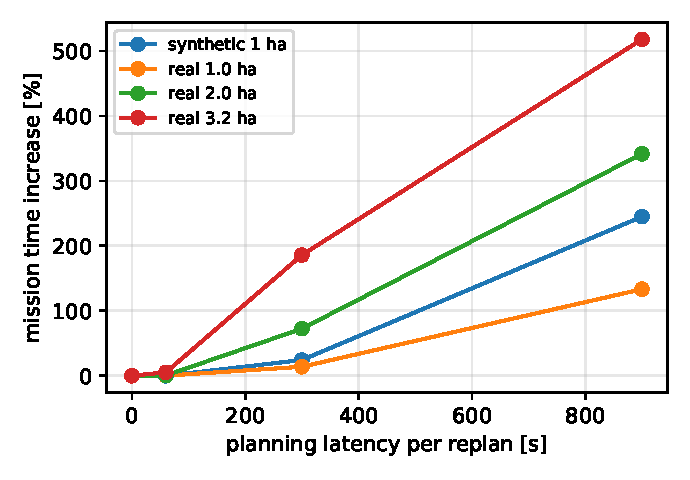
\includegraphics[width=0.62\textwidth]{figs/fig_latency.pdf}
\caption{Her yeniden planlamaya sabit bir gecikme eklendiğinde görev süresindeki artış
(Tall Spindle bahçeleri, ilk ve seyrek toplama geçişi, beş tohum)}\label{fig:latency}
\end{figure}

Sıralı bahçelerde (tüm sonuçlar: \nameref{app:rows}) PSB-MT/R, görevleri
sıra bantlarına göre ortalama \HvRowblockRelMean\% (koşuların
\HvWinRowblock\% kadarında daha hızlı), açgözlü dağıtıma göre
\HvGreedyRelMean\% (\HvWinGreedy\%) ve yeniden planlama yapmayan aynı planlayıcıya
göre \HvStaticRelMean\% (\HvWinStatic\%) kısaltmıştır. Kümelenmiş analizde sıra
bantlarına göre süre farkı $\HqRowsRowblockTime$\% iken olgun meyve/saat farkı
$\HqRowsRowblockThroughput$\% olmuştur; süre farkının güven aralığı sıfırı kapsamaktadır.
Yeniden planlama başına 1\,s süre verilen OR-Tools'un görevleri \HvOrtoolsOneRelMean\%
daha uzun sürmüş (PSB-MT/R, koşuların \HvWinOrtoolsOne\% kadarında daha hızlı);
kümelenmiş süre ve verimlilik farkları $\HqRowsOrtoolsOneTime$\% ve
$\HqRowsOrtoolsOneThroughput$\% olmuştur. Yeniden planlama başına 10\,s verildiğinde OR-Tools,
1\,ha'lık iki bahçede PSB-MT/R ile benzer ortalama sonuç vermiş (\HvOrtoolsOneZeroRelMean\%),
ancak bunu on kat planlama süresiyle sağlamıştır.

\paragraph{Planlama gecikmesi} Bir platform kasa değişimi için ortalama
\HvReplanGapMin{} dakikada bir dönmüş (koşular üzerinden medyan) ve her dönüş bir yeniden planlamayı tetiklemiştir.
Şekil~\ref{fig:latency}'de her PSB-MT/R planına yapay bir gecikme eklenmiştir. Bir dakikaya kadar
olan gecikmeler en fazla yüzde birkaçlık bir kayba yol açmış, ancak gecikme dönüşler arasındaki
aralığı aştığında planlar kuyrukta birikmiş ve görev süreleri hızla artmıştır (3.2\,ha'lık bahçede
300\,s gecikme için \HvLatOsmThreehaThreeZeroZero\%). PSB-MT/R'nin plan başına hesaplama süresi \HvPsbPlanMs\,ms olmuştur.

\subsection{Görselleştirme}
Benzetim kayıtları üç boyutlu bir Blender sahnesinde görsel olarak yeniden oynatılmıştır
(Şekil~\ref{fig:blender}): ağaç konumları, çeşitler, ağaç başına meyve sayıları,
platform yolları ve durakları, her durakta toplanan meyveler ve bölgeler kayıttan alınmış;
ağaç, elma, platform ve drone modelleri ise temsilî niteliktedir
(CC0 fotogrametri varlıkları ve gerçek ölçekte prosedürel modeller). Aynı sahne
üreteciyle eksiksiz bir görevin açıklayıcı bir videosu da üretilmiştir.
